\documentclass[dvisvgm]{standalone}

\usepackage{amsmath}
\usepackage[usenames,dvipsnames]{xcolor}
\usepackage{amsmath}
\usepackage{tikz}

\tikzset{
    new/.style={draw, fill=red!60, circle},
    base/.style={draw, circle},
}

\begin{document}
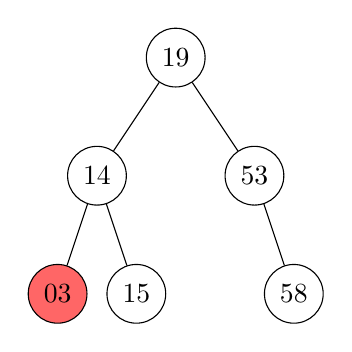
\begin{tikzpicture}
    [level 1/.style={sibling distance=20mm},
     level 2/.style={sibling distance=10mm}]
    \node[base] {19}
        child{node[base] {14}
            child{node[new] {03}}
            child{node[base] {15}}}
        child{node[base] {53}
            child[white]
            child{node[base] {58}}};
\end{tikzpicture}

\end{document}
